%%%%%%%% ICML 2021 EXAMPLE LATEX SUBMISSION FILE %%%%%%%%%%%%%%%%%

\documentclass{article}

% Recommended, but optional, packages for figures and better typesetting:
\usepackage{microtype}
\usepackage{graphicx}
\usepackage{subfigure}
\usepackage{booktabs} % for professional tables
\usepackage{amsmath,amsthm,amssymb,mathrsfs}
\usepackage{setspace}


\newcommand{\R}{\mathbb{R}}
\newcommand{\E}{\mathbb{E}}
\newcommand{\I}{\mathbb{I}}
\newcommand{\mle}{\textrm{mle}}
\DeclareMathOperator{\argmax}{argmax}

\newtheorem{theorem}{Theorem}
\newtheorem{lemma}{Lemma}

\newcommand{\com}[1]{\marginpar{{\begin{minipage}{0.33\textwidth}{\setstretch{1.1} \begin{flushleft} \footnotesize \color{red}{#1} \end{flushleft} }\end{minipage}}}}

\newcommand{\cvec}[2]
{
\left[\begin{array}{c}
#1 \\ #2 
\end{array}\right] 
}

\newcommand{\symmat}[3]
{
\left[\begin{array}{cc}
#1 & #2 \\ #2 & #3
\end{array}\right] 
}

\makeatletter
\newcommand{\subalign}[1]{%
  \vcenter{%
    \Let@ \restore@math@cr \default@tag
    \baselineskip\fontdimen10 \scriptfont\tw@
    \advance\baselineskip\fontdimen12 \scriptfont\tw@
    \lineskip\thr@@\fontdimen8 \scriptfont\thr@@
    \lineskiplimit\lineskip
    \ialign{\hfil$\m@th\scriptstyle##$&$\m@th\scriptstyle{}##$\hfil\crcr
      #1\crcr
    }%
  }%
}
\makeatother

% hyperref makes hyperlinks in the resulting PDF.
% If your build breaks (sometimes temporarily if a hyperlink spans a page)
% please comment out the following usepackage line and replace
% \usepackage{icml2021} with \usepackage[nohyperref]{icml2021} above.
\usepackage{hyperref}

% Attempt to make hyperref and algorithmic work together better:
\newcommand{\theHalgorithm}{\arabic{algorithm}}

% Use the following line for the initial blind version submitted for review:
%\usepackage{icml2021}

% If accepted, instead use the following line for the camera-ready submission:
\usepackage[accepted]{icml2021}

% The \icmltitle you define below is probably too long as a header.
% Therefore, a short form for the running title is supplied here:
\icmltitlerunning{Off-Policy Confidence Sequences}


\begin{document}

\twocolumn[
\icmltitle{Off-Policy Confidence Sequences}

% It is OKAY to include author information, even for blind
% submissions: the style file will automatically remove it for you
% unless you've provided the [accepted] option to the icml2021
% package.

% List of affiliations: The first argument should be a (short)
% identifier you will use later to specify author affiliations
% Academic affiliations should list Department, University, City, Region, Country
% Industry affiliations should list Company, City, Region, Country

% You can specify symbols, otherwise they are numbered in order.
% Ideally, you should not use this facility. Affiliations will be numbered
% in order of appearance and this is the preferred way.
\icmlsetsymbol{equal}{*}

\begin{icmlauthorlist}
\icmlauthor{Nikos Karampatziakis}{d365}
\icmlauthor{Paul Mineiro}{msr}
\icmlauthor{Aaditya Ramdas}{cmu}
\end{icmlauthorlist}

\icmlaffiliation{d365}{Microsoft Azure AI}
\icmlaffiliation{msr}{Microsoft Research}
\icmlaffiliation{cmu}{Carnegie Mellon University}

\icmlcorrespondingauthor{Nikos Karampatziakis}{nikosk@microsoft.com}

% You may provide any keywords that you
% find helpful for describing your paper; these are used to populate
% the "keywords" metadata in the PDF but will not be shown in the document
\icmlkeywords{Off-Policy Evaluation, Confidence Sequences}

\vskip 0.3in
]

% this must go after the closing bracket ] following \twocolumn[ ...

% This command actually creates the footnote in the first column
% listing the affiliations and the copyright notice.
% The command takes one argument, which is text to display at the start of the footnote.
% The \icmlEqualContribution command is standard text for equal contribution.
% Remove it (just {}) if you do not need this facility.

\printAffiliationsAndNotice{}  % leave blank if no need to mention equal contribution
%\printAffiliationsAndNotice{\icmlEqualContribution} % otherwise use the standard text.

\begin{abstract}
We develop confidence bounds that hold uniformly over time 
for off-policy evaluation in the contextual bandit
setting. These confidence sequences are based 
on recent ideas from martingale analysis and
are non-asymptotic, non-parametric, and valid 
at arbitrary stopping times. 
We provide algorithms for computing these 
confidence sequences that strike a 
good balance between computational and
statistical efficiency.
We empirically demonstrate the tightness
of our approach
in terms of failure probability and 
width and apply it to the problem of
off-policy model selection.
\end{abstract}

\section{Introduction}
Reasoning about the reward that 
a new policy $\pi$ would have achieved if it had been
deployed, a task known as Off-Policy Evaluation (OPE),
is one of the key technologies in Contextual
Bandits~\cite{epochgreedy} and Reinforcement Learning (RL).
A typical OPE use case is the validation of new modeling ideas
by data scientists. If OPE suggests that 
$\pi$ is better, this can then be validated 
online by deploying the new policy to the real world.

The classic way to to answer whether $\pi$ has better 
reward than the current policy $h$ is via a
confidence interval (CI).
%Move this to related work
%Several CIs have been proposed for OPE, both 
%finite-sample~\cite{thomas2015high} and 
%asymptotic~\cite{li2015counterfactual,karampatziakis2019empirical} ones.
Unfortunately, CIs take a very static view of the world.
Suppose that $\pi$ is better than $h$ 
and our OPE shows a higher but not significantly better 
estimated reward. What should we do? Since a CI holds for a
particular sample size and is not designed to handle 
interactive data collection, naively reapplying the CI
invalidates its coverage guarantee. While there are ways
to fix this (such as a crude union bound over time), 
the proper tool for such cases
are Confidence Sequences (CSs). A CS is a sequence 
of CIs such that the probability that they ever exclude 
the true value is bounded by a pre-specified quantity. 
Thus they allow for
optional (early) stopping and continuation 
(collecting more data).

In this work we develop CSs for OPE using 
recent insights from martingale analysis. 
Besides the aforementioned high probability
uniformly over time guarantee, these CSs make no parametric 
assumptions and are easy to compute. This
allows us to envision an \emph{off-policy A/B test}:
Instead of deploying $\pi$ directly 
we keep it in a staging area where 
we compute its off-policy CS as $h$ is collecting data.
Then $\pi$ can replace $h$ when (if ever)
$\pi$'s lower CS bound (LCS) 
overtakes the upper CS bound (UCS) of $h$.

We now introduce some notation to give 
context to our contributions.
We have contextual bandit data of the form $(x,a,r)$
collected by a historical policy $h$ in the following way:
First an $x$ was sampled from an unknown distribution $D$. 
Then $h$ assigns a probability to each action. 
An action $a$ is sampled with probability $h(a;x)$
and performed. A reward $r$ associated with performing $a$ in
situation $x$ is sampled from an unknown distribution $R(x,a)$. 
We now wish to know the reward of another policy $\pi$. We have
\begin{equation}
\label{eq:change-of-measure}
V(\pi) = \E_{\subalign{x&\sim D\\a&\sim\pi(x)\\r&\sim R(x,a)}}[r]
=
\E_{\subalign{x&\sim D\\a&\sim h(x)\\r&\sim R(x,a)}}\left[\frac{\pi(a;x)}{h(a;x)}r\right]
\end{equation}
where the second quantity can be estimated from 
data.%
%\footnote{We assume absolute continuity $\pi \ll h$ 
%as typical in OPE} 
Letting $w=\frac{\pi(a;x)}{h(a;x)}$  we see that 
$\E_{x\sim D,a\sim h}[w]=1$
(to reduce notation 
clutter we write $w$ instead of $w(x,a)$). More generally 
for any function $q(x,a)$ (typically
a predictor of the reward of $a$ at $x$)
\begin{equation}
\label{eq:control-variate}
\E_{x\sim D,a\sim h}[w q(x,a)] = \sum_{a'} \pi(a';x) q(x,a')    
\end{equation}
which leads to $\E[w]=1$ when $q(x,a)=1$ always. Eq.~\eqref{eq:change-of-measure} and \eqref{eq:control-variate}
are the building blocks of OPE estimators.
The IPS estimator \cite{HT52} estimates
\eqref{eq:change-of-measure} via Monte Carlo: $\hat{V}^{\textrm{IPS}}(\pi) = 1/n \sum_{i=1}^n w_i r_i $.
A plethora of other OPE estimators are discussed in Section~\ref{sec:related}. In general there is
a tension between the desirability of an unbiased estimator
like $V^{\textrm{IPS}}$ and the difficulty of working with it
with finite samples due to its excessive variance.

%Move to related work
%Doubly robust \cite{RnR, dudik2011doubly} incorporates \eqref{eq:control-variate}
%in \eqref{eq:change-of-measure} as an additive control variate
%while SNIPS \cite{swaminathan2015self} incorporates $\E[w]=1$ 
%as a multiplicative control variate. 

Recently, \cite{kallus2019intrinsically} proposed an OPE estimator 
based on Empirical Likelihood~\cite{owen2001empirical} with several
desirable properties. Empirical Likelihood (EL) has also been used to 
derive CIs for OPE in CBs \cite{karampatziakis2019empirical} 
and RL \cite{dai2020coindice}. Our CSs can be thought of as a natural 
extension to the online setting of the CIs 
for OPE in the batch setting. However our approach 
has several advantages
\begin{itemize}
\item Our results hold in finite samples and are
time-uniform without union bounds or peeling techniques.
\item We do not make any assumptions either parametric 
or about the support of $w$ and $r$ beyond boundedness.
%Mover to related work
%(c.f.~\cite{cappe2013kullback} for example).  
%\cite{ramdas2020admissible} 
\item Our statements remain valid under optional 
continuation (collecting more data) and/or optional stopping.
\end{itemize}

\section{Background: OPE Confidence Intervals}
We start by reviewing OPE CIs from the perspective of \cite{karampatziakis2019empirical}. Their CI
is constructed by considering plausible distributions 
from a nonparametric family 
$\mathcal{Q}$ of distributions  $Q$
for random vectors $(w,r) \in [0,w_{\max}]\times [0,1]$ 
under the constraint $\E_Q[w]=1$. Let $Q_{wr}$ be 
the probability that $Q \in \mathcal{Q}$ assigns to the event
where the importance weight is $w$ and the
reward is $r$. Then there exists $Q^* \in \mathcal{Q}$ such that
\[
Q^*_{wr}=\E_{x\sim D,a\sim h,\rho\sim R(x,a)}
\left[
\I\left[\frac{\pi(a;x)}{h(a;x)}=w\right]\cdot
\I\left[\rho=r\right]
\right]
\]
and 
$
V(\pi)=\E_{Q^*}[wr]
$.
To estimate of $V(\pi)$ we can find 
$Q^{\mle} \in \mathcal{Q}$ that maximizes
the data likelihood. To find a CI
we minimize/maximize $\E_Q[wr]$ over plausible 
$Q \in \mathcal{Q}$ so the data likelihood 
is not far off from that of $Q^{\mle}$.

Using convex duality the MLE is
$
Q^{\mle}_{wr} = \frac{1}{n(1+\lambda_1^{\mle}(w-1))}
$
where $\lambda_1^{\mle}$ is a dual variable solving
\[
\lambda_1^{\mle} = \argmax_{\lambda_1} \sum_{i=1}^n \log(1+\lambda_1(w_i-1))
\]
subject to $1+\lambda_1(w_{\max}-1)\geq 0$, $1-\lambda_1\geq 0$.
The profile likelihood
$
L(v)=\sup_{Q: \E_Q[w]=1, \E_Q[wr]=v} \prod_{i=1}^n Q_{w_i,r_i}
$
is used for CIs. From EL theory,
an asymptotic $1-\alpha$-CI is
\[
\left\{v: -2\ln\left(\frac{\prod_{i=1}^n Q^{\mle}_{w_i,r_i}}{L(v)}\right)
\leq \chi_1^{2,1-\alpha}\right\}
\]
where $\chi_1^{2,1-\alpha}$ is the $1-\alpha$ quantile of a $\chi^2$
distribution with 1 degree of freedom.
Again using convex duality the CI is
\[
\left\{v: 
B(v)-\sum_{i=1}^n\log(1+\lambda_1^{\mle}(w_i-1))
\leq \chi_1^{2,1-\alpha}\right\}
\]
where the dual profile log likelihood $B(v)$ is
\begin{equation}
B(v) = \sup_{\lambda_1,\lambda_2} \sum_{i=1}^n \log(1+\lambda_1(w_i-1)+\lambda_2(w_i r_i -v))    \label{eq:dual-lik}
\end{equation}
subject to $(\lambda_1,\lambda_2) \in \mathcal{D}_v^0$ where 
\begin{align}
\mathcal{D}_v^{m} =
\{(\lambda_1,\lambda_2): & 1+\lambda_1(w-1)+\lambda_2(wr-v)\geq m \label{eq:batch-domain}\\
                         & \forall (w,r) \in \{0,w_{\max}\}\times \{0,1\} \notag
\}.
\end{align}
The CI endpoints can be found via 
bisection on $v$.

\section{Off-policy Confidence Sequences}
We now move from the batch setting and asymptotics to
online procedures and finite sample statements.
We adapt and extend ideas from \cite{waudby-smith_variance-adaptive_2020}.
The key insight is to interpret the 
dual log likelihood \eqref{eq:dual-lik}
as the log wealth accumulated by a skeptic who is betting against the
hypotheses 
\[
\E_{Q^*}[w]=1 \text{ and } \E_{Q^*}[wr]=v.
\]
In particular,
the skeptic starts with a wealth of $1$ and wants to 
maximize her wealth. Her bet on the outcome $w-1$ is captured by $\lambda_1$, while $\lambda_2$
represents the bet on the outcome of $wr-v$ so that the wealth after
the $i$-th sample is multiplied by $1+\lambda_1(w_i-1)+\lambda_2 (w_i r_i -v)$. If the outcomes had been in $[-1,1]$ then
$|\lambda_1|$ and $|\lambda_2|$ would have an interpretation as 
the fraction of the skeptic's wealth that is being risked 
on each step. The bets can be positive
or negative, and their signs represent the directions of the bet. For example, $\lambda_2<0$ means 
the skeptic will make money if $w_ir_i-v<0$.
Enforcing the constraints 
\eqref{eq:batch-domain}
from the batch setting here means that 
the resulting wealth cannot be negative.


The first
benefit of this framing is that we have 
mapped the abstract concepts of dual likekihood,
dual variables, and dual constraints to more familiar 
concepts of wealth, bets, and avoiding bankruptcy. 
We now formalize our constructions and
show how they lead to always valid, finite sample, 
CSs. We introduce a family of processes
\[
K_t(v) = \prod_{i=1}^t (1+\lambda_{1,i} (w_i-1) +\lambda_{2,i}(w_i r_i - v))
\]
where $\lambda_{1,i}$ and $\lambda_{2,i}$ are predictable, i.e. measurable
with respect to the sigma field $\sigma(\{(w_j,r_j)\}_{j=1}^{i-1})$.
We now state two key properties of the process $K_t(V(\pi))$.
\begin{theorem}
\label{thm:martingale}
$K_t(V(\pi))$ is a non-negative martingale.
\end{theorem}
\begin{theorem}
\label{thm:ville}
$\Pr(\exists t: K_t(V(\pi)) \geq \frac{1}{\alpha})\leq \alpha$
$\forall \alpha \in [0,1]$
\end{theorem}
%Move to appendix
%Proposition 1: . Proof sketch:
%Conditioning on all history up to 
%$t-1$, the first $t-1$ factors in the product are fixed and so are %$\lambda_{1,t}$ and $\lambda_{2,t}$. The terms multiplying %$\lambda_{1,t}$ and $\lambda_{2,t}$ are zero mean
%so we end up with $\E[K_t|\mathcal{H}_{t-1}] = K_{t-1}$
All proofs are in the appendix.
Now our goal is clearer. The process $K_t(v)$ tracks the wealth
of a skeptic betting against
$V(\pi)=v$. The process $K_t(V(\pi))$ is a martingale so it has
a small probability of attaining large values. For other values 
of $v$, a series of good bets can force $K_t(v)$ to eventually
be large. How to best set these bets is the subject of what follows.
Regardless of how the bets are set we have
\begin{theorem}
\label{thm:cs}
The sequence $C_t = \{v:K_t(v)\leq \frac{1}{\alpha}\}$ is a $1-\alpha$ confidence sequence for $V(\pi)$.
\end{theorem}
The strength of our approach comes from these results, as they 
guarantee always valid bounds for $V(\pi)$ using only martingale
arguments crucially avoiding parametric or other assumptions.

\section{Betting Strategies}

\subsection{Follow The Leader}
In \cite{waudby-smith_variance-adaptive_2020} the authors develop
an array of increasingly more effective betting procedures. 
Some of the most effective ones find the bet that would in hindsight
result in maximum wealth (SOS) or an approximation thereof (aSOS).
This approach is also known as Follow-The-Leader (FTL) and is 
known to incur constant regret for iid 
problems~\cite{de2014follow}.
Our first proposed strategy 
is therefore FTL where we set the 
bets $\lambda_1$ and $\lambda_2$ to maximize the wealth in hindsight
by solving
\begin{equation}
\lambda_{t}^{\textrm{ftl}}(v) = \argmax_{\lambda} \sum_{i=1}^{t-1} \ln(1+\lambda_1 (w_i-1)+\lambda_2(w_i r_i - v)) \label{eq:ftl}
\end{equation}
for every step of betting in $K_t(v)$. 
We note that FTL is not robust 
to deviations from the iid assumption and 
can incur linear regret. While this is 
beyond the scope of this paper, if 
the iid assumption is questionable we can feed
the exp-concave losses 
$\ell_i(\lambda) = 
-\ln(1+\lambda_{1}(w_i - 1)+\lambda_{2}(w_i r_i - v))$
to an online algorithm such as ONS 
to compete against the best fixed bet in hindsight.
The problem~\eqref{eq:ftl} is convex and can be solved in polynomial time
leading to an overall polynomial time algorithm. However,
this approach has two undesirable properties. First, the 
algorithm needs to store the whole history of $(w,r)$ samples
and second the overall algorithm is tractable but slow.
In the rest of the section we propose techniques that trade off
statistical for computational efficiency.

\subsection{Maximizing a lower bound on wealth}

We can avoid having to store all history by optimizing
an easy to maintain lower bound of \eqref{eq:ftl}.
We use the lemma
\begin{lemma} 
\label{lem:quadbound}
For all $x\geq -\frac{1}{2}$ and $\psi=2-4\ln(2)$, we have
\[
\ln(1+x)\geq x + \psi x^2.
\]
\end{lemma}
%Move to appendix
%The proof is straightforward by checking that the boundary $x=-\frac{1}{2}$ and all critical points of $f(x) = \ln(1+x)- x - \psi x^2$ evaluate to non-negative quantities. 
Observe that if we restrict our bets to lie in the convex set
$\mathcal{D}_v^{1/2}$ (cf.~eq.~\eqref{eq:batch-domain})
then for all $\lambda \in \mathcal{D}_v^{1/2}$
\begin{align*}
\sum_{i=1}^{t-1} \ln(1+\lambda_1 (w_i-1)+\lambda_2(w_i r_i - v)) 
\geq
\lambda^\top \sum_{i=1}^{t-1} b_i(v) \\
+\psi \lambda^\top \left(\sum_{i=1}^{t-1} A_i(v)\right) \lambda \\ 
\end{align*}
where 
$b_i(v)=
\left[\begin{array}{c} 
w_i-1 \\ w_i r_i -v 
\end{array}\right] 
$
and 
$
A_i(v) = b_i(v)b_i(v)^\top.
$
The first step towards a more efficient algorithm is to 
set our bets at time $t$ as
\begin{equation}
\lambda_t(v) = \argmax_{\lambda \in \mathcal{D}_{v}^{1/2}}
\psi  \lambda^\top \left(\sum_{i=1}^{t-1} A_i(v)\right) \lambda 
+ \lambda^\top \sum_{i=1}^{t-1} b_i(v).
\label{eq:quadoptv}
\end{equation}
The restriction $\lambda \in \mathcal{D}_{v}^{1/2}$ 
is very mild: it does 
not allow the skeptic to bet in ways that would cause her 
to lose more than half of her wealth from any single outcome.
The first advantage of this formulation is that 
$\sum_i A_i(v)$ and $\sum_i b_i(v)$ are low degree 
polynomials of $v$ and can share the coefficients
    \begin{align*}
        \sum_{i=1}^{t-1} A_i(v) &= 
        A_t^{(0)} + v A_t^{(1)} + v^2 A_t^{(2)}\\   
        \sum_{i=1}^{t-1} b_i(v) &= b_t^{(0)} + v b_t^{(1)}.  
    \end{align*}
Secondly, the coefficients can be updated incrementally
    \begin{align}
        A_t^{(0)} &=\sum_{i=1}^{t-1}\symmat{(w_i-1)^2}{(w_i-1)w_i r_i}{w_i^2r_i^2} \label{eq:upsuffa0}\\
        A_t^{(1)} &= \sum_{i=1}^{t-1} \symmat{0}{-(w_i-1)}{-2w_ir_i}\\
        A_t^{(2)} &=\sum_{i=1}^{t-1}  \symmat{0}{0}{1}\\
        b_t^{(0)} &=\sum_{i=1}^{t-1}  \cvec{w_i-1}{w_ir_i}\\
        b_t^{(1)} &=\sum_{i=1}^{t-1}  \cvec{0}{-1}. \label{eq:upsuffb1}
    \end{align}
Finally, maximization can be done very efficiently since there are 
only four constraints and two variables. In our implementation, we
first try to return the unconstrained maximizer, if feasible. 
If not, we evaluate the objective on up to 8 candidates: 
up to one candidate per face of the polytope $\mathcal{D}_v^{1/2}$ 
(obtained via maximizing the objective subject to one equality constraint) 
and its 4 vertices.

\subsection{Common Bets and Hedging}
The most competitive betting sequences for the process
$K(v)$ will take advantage 
of the knowledge of $v$. However, placing different
bets for different values of $v$ creates two problems:
First, the resulting confidence set need not be an 
interval and second makes it hard 
to implement Theorem~\ref{thm:cs} 
in a computationally efficient way.
Indeed, even in the simpler setup of
\cite{waudby-smith_variance-adaptive_2020}
the authors maintain a grid of test values 
for the quantity of interest (here $v$)  
and at least keep track of the wealth separately.
This is because tracking the wealth for each
value in the grid is not straightforward when
the bets are different. 

To make wealth tracking easy and
obtain algorithms that do not require the 
discretization of the domain of $v$, a natural
proposal would be to use a common bet for 
all $v$ in each timestep. Unfortunately, 
this is not adequate because we do need 
$\lambda_2 > 0$ for $v<\E_{Q^*}[wr]$ 
and $\lambda_2 < 0$ for $v>\E_{Q^*}[wr]$. 
A simple fix is to use a hedged 
strategy as in~\cite{waudby-smith_variance-adaptive_2020}.
First, we split our initial wealth equally.
We use the first half to bet against low $v$'s
via the wealth process
\[
K_t^{+}(v) = \prod_{i=1}^t \left(1+\lambda_{1,i}^{+}(w_i-1)+\lambda_{2,i}^{+}(w_i r_i -v)\right)
\]
and the second half to bet against high $v$'s
via a separate process $K_t^{-}(v)$ which 
for symmetry we parametrize as
\begin{equation}
K_t^{-}(v) = \prod_{i=1}^t \left(1+\lambda_{1,i}^{-}(w_i-1)+\lambda_{2,i}^{-}(w_i r'_i -v'\right).
\label{eq:wealth-minus} 
\end{equation}
where $r'_i=1-r_i$ and $v'=1-v$.
Eq.~\eqref{eq:wealth-minus} 
can be seen as the wealth process for betting against $1-v$ 
in an world where all rewards $r$ have been remapped 
to $1-r$. Thus betting against high values of $v$ 
reduces to betting against low values of $v$ in a
modified process. 

The total wealth of the hedged process is:
\begin{equation}
K_t^{\pm}(v) = \frac{1}{2} (K_t^{+}(v) + K_t^{-}(v))
\label{eq:hedged}
\end{equation}
and can be used in the same way as $K_t(v)$
\begin{theorem}
$K_t^{\pm}(V(\pi))$ is a non-negative martingale
\end{theorem}

It remains to specify how to design a common bet
for $K_t^{+}(v)$.
Betting against any fixed $v_0$ 
will not work well when $V(\pi)=v_0$
since the optimal bet for $V(\pi)$ is 0 but
such a bet cannot help us reject those $v$ that are far from
$V(\pi)$. Therefore we propose to adaptively choose
the bets against the smallest $v$ 
that has not been rejected. As we 
construct the confidence sequence, and its running 
intersection, we have access to the values of $v$
that constitute the endpoints of the confidence sequence
at the last time step. These values are on the cusp of
plausibility given the available data and confidence level
which means the bets are neither too conservative nor 
too detached from what can be estimated.
\begin{figure*}
    \centering
    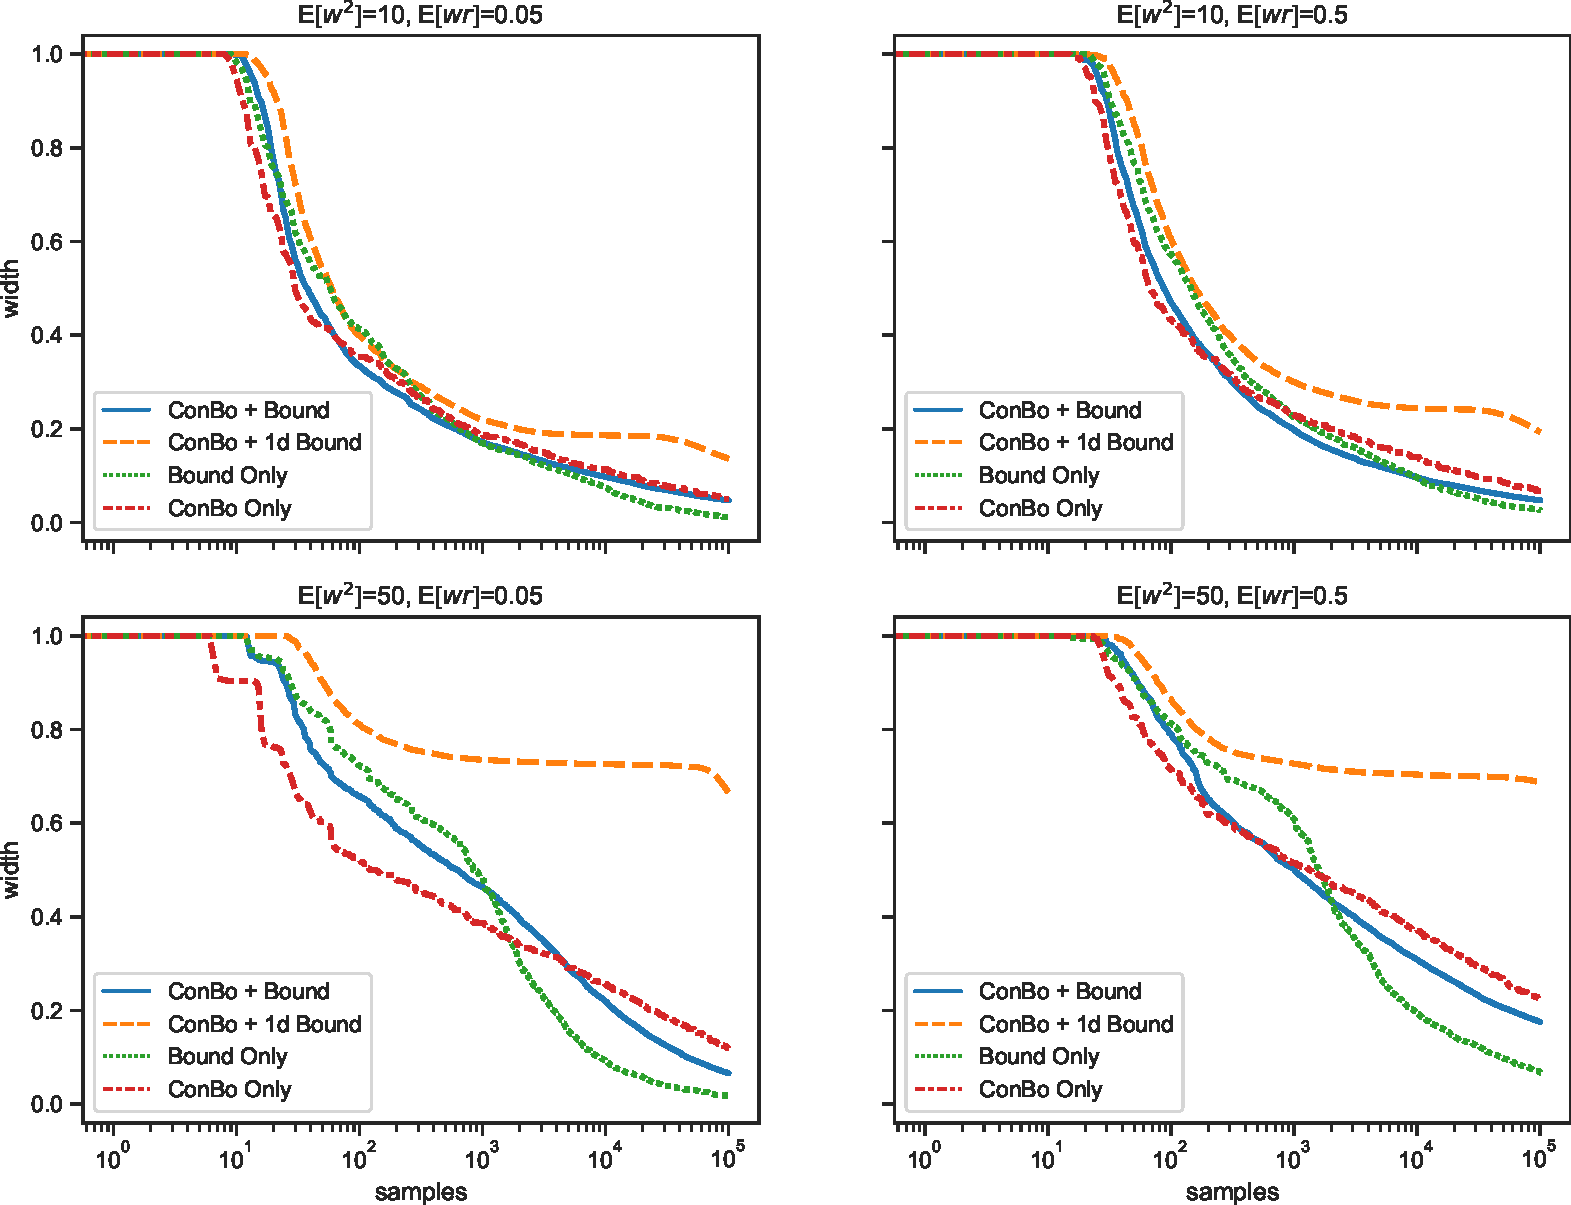
\includegraphics[width=0.8\textwidth]{width}
    \caption{Caption}
    \label{fig:my_label}
\end{figure*}

\subsection{Avoiding grid search}

Once we have determined $v$ for the current step we could 
choose $\lambda$ via \eqref{eq:quadoptv}. For reasons 
that will become apparent shortly, we can also consider
\begin{equation}
\lambda_t = \argmax_{\lambda \in \mathcal{C}}
\psi  \lambda^\top \left(\sum_{i=1}^{t-1} A_i(v)\right) \lambda 
+ \lambda^\top \sum_{i=1}^{t-1} b_i(v).
\label{eq:quadopt}
\end{equation}
where $\mathcal{C}=\left\{\lambda: \lambda_2\geq 0, 
\lambda_1 + \lambda_2 \leq \frac{1}{2},
\lambda_1 \left(w_{\max}-1\right) \geq \lambda_2 -\frac{1}{2}
\right\}$ is the intersection of $\mathcal{D}_{v}^{1/2}$ 
(eq.~\eqref{eq:batch-domain}) for all $v \in [0,1]$ 
and the constraint $\lambda_2\geq 0$ which we expect
from good bets when $\E[wr-v]>0$. 

Given $\lambda_1,\ldots,\lambda_{t-1}$, we get from Lemma~\ref{lem:quadbound} 
\[
\sum_{i=1}^{t-1} \ln(1+\lambda_{1,i} (w_i-1)+\lambda_{2,i} (w_i r_i - v)) 
\geq
\psi  
 \sum_{i=1}^{t-1} \lambda_i^\top A_i(v)\lambda_i  +  \sum_{i=1}^{t-1} \lambda_i^\top b_i(v)
\]
for all $v \in [0,1]$. Thus, if the lower bound exceeds $\ln(1/\alpha)$ 
for a particular $v$, the log wealth will also exceed it. Furthermore,
the lower bound is quadratic in $v$ so we can easily find those values
$v \in [0,1]$ such that
\begin{equation}
   \psi  
 \sum_{i=1}^{t-1} \lambda_i^\top A_i(v)\lambda_i  +  \sum_{i=1}^{t-1} \lambda_i^\top b_i(v) = \ln\left(\frac{2}{\alpha}\right) 
 \label{eq:quadv}
\end{equation} 
The extra $2$ is due to the hedged process. 
Appendix~\ref{app:nogrid2d} contains the details and 
how to incrementally maintain statistics for solving
\eqref{eq:quadv} via eqs.~\eqref{eq:upsuffc}-\eqref{eq:upsuffu}.
The advantage of \eqref{eq:quadopt}
over \eqref{eq:quadoptv} is that the latter cannot 
ensure that old bets will produce values in $C_v$ for 
future values of $v$ while the former always does.

The whole process of updating the statistics,
tightening the lower bound $v$ via \eqref{eq:quadv}
and computing the new bets via \eqref{eq:quadopt}
is summarized in Algorithm~\ref{alg:main}.



\begin{algorithm}[tb]
   \caption{Efficient Betting}
   \label{alg:main}
\begin{algorithmic}
    \STATE {\bfseries Input:} process $Z=(w_i,r_i)_{i=1}^\infty, w_{\max}, \alpha$
    \STATE Let $Z' = (w_i,1-r_i)$ for $(w_i,r_i)$ in $Z$
    \FOR{$v_i,v_i'$ in zip(LCS($Z$), LCS($Z'$))}
        \STATE Output($v_i,1-v_i'$)
   \ENDFOR
\FUNCTION{LCS($Z$)}{
    \STATE $\lambda_1 = [0,0]^\top, v = 0$
    \FOR{$i=1,\ldots$}
        \STATE Observe $(w_i,r_i)$ from $Z$
        \STATE Update statistics via \eqref{eq:upsuffa0}-\eqref{eq:upsuffb1} and \eqref{eq:upsuffc}-\eqref{eq:upsuffu}.
        \IF{\eqref{eq:quadv} has real roots}
            \STATE $v=\max(v, \textrm{largest root of }\eqref{eq:quadv})$
        \ENDIF
        \STATE \textbf{yield} $v$
        \COMMENT{execution suspends/resumes here}
        \STATE $A = A_i^{(0)} +v A_i^{(1)} + v^2 A_i^{(2)}$
        \STATE $b = b_i^{(0)} +v b_i^{(1)}$
        \STATE  $\lambda_{i+1} = \argmax_{\lambda \in C}  \lambda^\top \psi A \lambda+  b^\top \lambda$.
    \ENDFOR
    }
\ENDFUNCTION
\end{algorithmic}
\end{algorithm}

\section{Related Work}
\label{sec:related}

\section{Experiments}



\subsection{Coverage} \label{sec:coverage}
While Theorem~\ref{thm:cs} says that any predictable betting sequence
guarantees correct coverage, some will overcover to a greater extent than others. Here we investigate the coverage properties of our 
proposal. We generate 1000 sequences of 100000 $(w,r)$ pairs 
each from a different distribution. All distributions are 
maximum entropy distributions subject to
support $(w,r) \in \{0, 0.5, 2, 100\} \times \{0,1\}$,
$\E[w]=1$, $\E[w^2]=10$ and $V(\pi)$ sampled uniformly 
in $[0,1]$. In Figure X we show the 
empirical mean coverage of the confidence sequences produced 
by Algorithm~\ref{alg:main} with $\alpha=0.05$. 


\subsection{Computational vs. Statistical Efficiency}
To investigate the design choices we proposed we consider
four synthetic environments which are just 
distributions over $(w,r)$ pairs. The four environments
are generated in the same way a section~\ref{sec:coverage}
but with $(V(\pi),\E[w^2]) \in \{0.05, 0.5\} \times \{10, 100\}$

Comparison candidates: There's really nothing that does 
the same. Compare with on-policy CS? 
Compare with fixed $n$ CIs?
Compare with running a CI for each $t$ with budget 
$\alpha/(t(t+1))$?
Comparison aspect: length of interval as a function of time.
\subsubsection{Separate betting sequences}
Compare our proposed procedure with solving a different QP based on 
the value of $v$ for a fine grid of values.
\subsubsection{Exactly maximizing wealth in hindsight}
Compare our proposed procedure with exactly maximizing wealth in hindsight.
\subsection{Is it necessary to use vector bets?}
Compare our procedure with one that uses one dimensional optimization.

Since $\E[w]=1$ no matter what, it seems that betting  on $w_i-1$ 
cannot have any long term benefits. Here we perform an experiment with a 
betting strategy that only bets on $w_i r_i -v$. It turns out however that
even with the best fixed $\lambda_2$ in hindsight (a strategy that does not lead 
to valid intervals but suggests what are the limits of what is achievable) 
shows that we can get a nice lower bound but the upper bound remains vacuous. 

To combat this we follow a hedged strategy. 
We show 
in~\ref{app:betaopt} that we can set $\lambda_1=\max(0,-\lambda_2)$ to minimize the worst case wealth loss at the next step.
Since we expect $\lambda_2>0$ for the lower bound and $\lambda_2<0$ 
for the upper bound our hedged strategy will 
split the wealth in 
half and set $\lambda_1=0$ for the lower bound and $\lambda_1=-\lambda_2$ 
for the upper bound. This leads to the wealth processes
\[
K_t^{+}(v)=\prod_{i=1} (1+\lambda_{2,i}^{+} (w_i r_i -v))
\]
and
\begin{equation}\label{eq:wealth-1d-minus}
K_t^{-}(v)=\prod_{i=1} (1+\lambda_{1,i}^{-}(w_i-1)+\lambda_{2,i}^{-} (v-w_i r_i))
=\prod_{i=1} (1+\lambda_{2,i}^{-} (w_i (1-r_i)-(1-v)))
\end{equation}
Eq.~\eqref{eq:wealth-1d-minus} 
can be seen as how we would bet to find (one minus) the 
lower bound in the case where all rewards $r$ have been remapped 
to $1-r$. The final process is 
\[
K_t(v)=\frac{1}{2}(K_t^{+}(v)+K_t^{-}(v))
\]
Remark: $\lambda_{2,i}^{-}$ in \eqref{eq:wealth-minus} can be at most $1/(1-v)$ so that the wealth remains positive. As a practical suggestion, one could truncate at $1/[2(1-v)]$.

\subsection{Maximizing a wealth lower bound}

We start with a simple inequality valid for $\xi\geq-1$ and 
$0\leq \lambda < 1$ (See \cite{fan2015exponential} Prop 4.1 for a proof within a proof)
\begin{equation}
\ln(1+\lambda \xi) \geq \lambda \xi+\left(\ln\left(1-\lambda\right)+\lambda\right)\cdot \xi^{2}
\label{eq:fanbound}
\end{equation}
in our case both $wr-v>-1$ and $w(1-r)-(1-v)>-1$ always.

Imagine we play the same $\lambda_2$ for each step. Then
\[
\ln(K_t^{+}(v)) \geq \lambda_2 \sum_i (w_i r_i -v) + \left(\ln\left(1-\lambda_2\right)+\lambda_2\right) \sum_i (w_i r_i -v)^2
\]
when $\sum_i (w_i r_i -v)^2>0$ the lower bound is concave and can 
be maximized in $\lambda_2$ by setting its derivative to 0. This gives
the optimal $\lambda_2$ in hindsight for the wealth lower bound 
\[
\lambda_2^* = \frac{\sum_i (w_i r_i -v)}{\sum_i (w_i r_i -v)+\sum_i (w_i r_i -v)^2}
\]
and $\lambda_2^*=0$ when $\sum_i (w_i r_i -v)^2=0$. A similar argument 
applies for $K_t^{-}(v)$.

The lower bound maximization betting strategy is different from 
the GROW strategy \cite{waudby-smith_variance-adaptive_2020} 
which is derived by approximating the optimal wealth up to now 
and playing the best fixed bet in hindsight for that approximation.

\com{Re GROW vs this: Not sure which is a better idea: in our experiments, they are empirically quite similar in terms of the resulting CS. This type of expression is also going to be in our updated paper, and is more similar and inspired by approximations to Online Newton Step (eg: Orabona and Cutosky, COLT 2018) rather than GROW/EL.}



\bibliography{opecs}
\bibliographystyle{unsrtnat}
\newpage
\onecolumn
\appendix
\section{Proofs}

\subsection{Proof of Theorem~\ref{thm:martingale}}
\subsection{Proof of Theorem~\ref{thm:ville}}
\subsection{Proof of Theorem~\ref{thm:cs}}
\subsection{Proof of Lemma~\ref{lem:quadbound}}
\section{Avoiding grid search}
\label{app:nogrid2d}
We first lower bound each process separately, then lower bound
the hedged process. We denote the bets for $K^{+}$ (respectively
$K^{-}$) as $\lambda^{+}$, (resp. $\lambda^{-}$).
From lemma~\ref{lem:quadbound} we have
\[
\ln(K_t^{+}(v)) \geq \sum_{i=1}^{t-1} {\lambda_i^{+}}^\top b_i(v) + \psi \sum_i {\lambda_i^{+}}^\top A_i(v) {\lambda_i^{+}}
\]
and
\[
\ln(K_t^{-}(v)) \geq \sum_{i=1}^{t-1} {\lambda_i^{-}}^\top b_i'(v') + \psi \sum_i {\lambda_i^{-}}^\top A_i'(v') {\lambda_i^{-}}
\]
where $v'=1-v$, 
$b_i'(v)=
\cvec{w_i-1}{w_i (1-r_i) -v}
$
and $A_i'(v)=b_i'(v)b_i'(v)^\top$.
For the Hedged process, using that for any $a,b$
\[
\ln\left(\exp(a)+\exp(b)\right)\geq \max(a,b)
\]
to first establish
\[
\ln(K^{\pm}(v)) \geq \max(\ln(K^{+}(v))-\ln(2),\ln(K^{-}(v))-\ln(2))
\]
and further bound each term in the maximum by the respective 
quadratic lower bound. We conclude that
if a $v$ achieves 
\[
 \sum_{i=1}^{t-1} {\lambda_i^{+}}^\top b_i(v) + \psi \sum_i {\lambda_i^{+}}^\top A_i(v) \lambda_i^{+} = \ln\left(\frac{2}{\alpha}\right)
\]
or a $v'=1-v$ achieves 
\[
\sum_{i=1}^{t-1} {\lambda_i^{-}}^\top b_i'(v') + \psi \sum_i {\lambda_i^{-}}^\top A_i'(v') \lambda_i^{-} = \ln\left(\frac{2}{\alpha}\right)
\]
then we also achieve $K_t^{\pm}(v) \geq \frac{1}{\alpha}$.
In terms of $v$ and $v'$ these expressions are second degree
equations and thus their real roots in $[0,1]$ (if any) provide 
a safe bracketing of the confidence region $\{v:K_t^{\pm}(v)\leq 1/\alpha\}$. For $K_t^{+}$ let
\begin{align}
C_t&= \sum_{i=1}^{t-1} {\lambda_i^{+}}^\top \cvec{w_i-1}{w_i r_i} \label{eq:upsuffc}\\
S_t&= \sum_{i=1}^{t-1} {\lambda_i^{+}}^\top \cvec{0}{1} \\
Q_t&= \sum_{i=1}^{t-1} \psi  {\lambda_i^{+}}^\top \symmat{(w_i-1)^2}{(w_i-1)w_i r_i}{w_i^2r_i^2} \lambda_i^{+} \\
T_t&= \sum_{i=1}^{t-1} \psi  {\lambda_i^{+}}^\top \symmat{0}{-(w_i-1)}{-2w_ir_i} \lambda_i^{+} \\
U_t&=  \sum_{i=1}^{t-1} \psi {\lambda_i^{+}}^\top \symmat{0}{0}{1} \lambda_i^{+} \label{eq:upsuffu}
\end{align}
and define $C_t',S_t',Q_t',T_t',U_t'$ similarly by using $\lambda_i^{-}$ 
instead of $\lambda_i^{+}$ and $1-r_i$ instead of $r_i$. Then
the largest real root $v^{+}$ of
\[
C_t - S_t v + Q_t + T_t v + U_t v^2 - \ln\left(\frac{2}{\alpha}\right) = 0,
\]
if it exists, satisfies $K_t^{\pm}(v^{+})\geq \frac{1}{\alpha}$. Similarly
we can obtain $v'$ as the largest real root of the quadratic
with $C_t',S_t',Q_t',T_t',U_t'$ in place of $C_t,S_t,Q_t,T_t,U_t$,
if it exists. Then $v^{-}=1-v'$ satisfies $K_t^{\pm}(v^{-})\geq \frac{1}{\alpha}$.



\section{A Scalar Betting Strategy}
\subsection{Elimination of one bet} \label{app:betaopt}
Since the $\lambda_1$ bet cannot provide any long-term benefit, its purpose can only be as a hedge in the short-term. We formulate this by considering the
worst case wealth reduction among three outcomes :
$(w,r)=(w_{\max},1)$, 
$(w,r)=(w_{\max},0)$ and $w=0$ with any reward. We require that $\lambda_1$
is set to maximize the wealth in the worst of these outcomes. Thus we set 
up a family of linear programs parametrized by $\lambda_2$ and $v$ and with optimization variables $\alpha$ and $\lambda_1$:
\begin{equation*}
\begin{array}{ll@{}ll}
\text{maximize}  & \alpha &\\
\text{subject to}& \alpha \leq 1+\lambda_1(w_{\max}-1)+\lambda_2(w_{\max}-v)  & &(z_1) \\
                 & \alpha \leq 1+\lambda_1(w_{\max}-1)-\lambda_2 v            & &(z_2) \\
                 & \alpha \leq 1-\lambda_1-\lambda_2 v                        & &(z_3) \\
\end{array}
\end{equation*}
Where the variable $z_i$ in parentheses next to each constraint is the corresponding dual variable. 
\begin{theorem}
For any  and any $v\in [0,1]$ and any $\lambda_2 \in \R$, the optimal value of $\lambda_1$ in the above LP is $\lambda_1^*=\max(-\lambda_2,0)$.
\end{theorem}
\begin{proof}
The dual program is
\begin{equation*}
\begin{array}{ll@{}ll}
\text{minimize}  & (1+\lambda_2(w_{\max}-v))z_1 +(1-\lambda_2 v) z_2 + (1-\lambda_2 v) z_3 &\\
\text{subject to}& z_i \geq 0  & i=1,2,3 \\
                 & -(w_{\max}-1)(z_1+z_2)+z_3 = 0 \\
                 & z_1+z_2+z_3=1 \\
\end{array}
\end{equation*}
Consider the following two dual feasible settings:
\[
z_1=0,z_2=\frac{1}{w_{\max}}, z_3=\frac{w_{\max}-1}{w_{\max}}
\]
and 
\[
z_1=\frac{1}{w_{\max}}, z_2=0, z_3=\frac{w_{\max}-1}{w_{\max}}
\]
with corresponding dual objectives: $1-\lambda_2 v$ and $1-\lambda_2 v + \lambda_2$. From here we see that if $\lambda_2 > 0$ the former attains a
better dual objective and is thus a better bound
for the primal objective. When $\lambda_2<0$ the latter
is better. 

When $\lambda_2>0$, a primal feasible setting is
$\alpha=1-\lambda_2 v,\lambda_1=0$. Furthermore this setting
achieves the same objective as the first dual feasible setting so 
we conclude that these are the optimal primal and dual solutions when $\lambda_2>0$.

When $\lambda_2<0$, a primal feasible setting is 
$\alpha=1-\lambda_2 v +\lambda_2, \lambda_1=-\lambda_2$. Furthermore this setting
achieves the same objective as the second dual feasible setting
so we conclude that these are the optimal primal and dual solutions when $\lambda_2<0$. 

Finally when $\lambda_2=0$ the two cases give the same value for $\lambda_1$ so we conclude $\lambda_1=\max(-\lambda_2,0)$ for all $\lambda_2 \in \R$ (and $v\geq 0$).
\end{proof}

\subsection{Avoiding grid Search}
Suppose that our bets $\lambda_2^{+}$ and $\lambda_2^{-}$ do not depend on $v$.
We have the individual lower bounds
\[
\ln(K^{+}(v)) \geq \sum_i \lambda_{2,i}^{+} (w_i r_i -v) + \sum_i (\ln(1-\lambda_{2,i}^{+})+\lambda_{2,i})(w_i r_i -v)^2
\]
and
\[
\ln(K^{-}(v)) \geq \sum_i \lambda_{2,i}^{-} (w_i r_i' -v') + \sum_i (\ln(1-\lambda_{2,i}^{-})+\lambda_{2,i}^{-})(w_i r_i' -v')^2
\]
where $r'=1-r$, $v'=1-v$.
For the Hedged process, using that for any $a,b$
\[
\ln\left(\exp(a)+\exp(b)\right)\geq \max(a,b)
\]
to first establish
\[
\ln(K^{\pm}(v)) \geq \max(\ln(K^{+}(v))-\ln(2),\ln(K^{-}(v))-\ln(2))
\]
and further bound each term in the maximum by the respective 
quadratic lower bound. We conclude that
if a $v$ achieves 
\[
\sum_i \lambda_{2,i}^{+} (w_i r_i -v) + \sum_i (\ln(1-\lambda_{2,i}^{+})+\lambda_{2,i}^{+})(w_i r_i -v)^2 = \ln\left(\frac{2}{\alpha}\right)
\]
or a $v'=1-v$ achieves 
\[
\sum_i \lambda_{2,i}^{-} (w_i r_i'-v') + \sum_i (\ln(1-\lambda_{2,i}^{-})+\lambda_{2,i}^{-})(w_i r_i' - v')^2
=\ln\left(\frac{2}{\alpha}\right)
\]
then we also achieve $K^{\pm}(v) > \frac{1}{\alpha}$. 
Thus, a valid confidence interval can be obtained by considering
the roots of these quadratics.  Let
\begin{align*}
C&=\sum_i \lambda_{2,i}^{+} w_i r_i & 
C'&=\sum_i \lambda_{2,i}^{-} w_i r_i'\\
S&=\sum_i \lambda_{2,i}^{+} & 
S'&=\sum_i \lambda_{2,i}^{-} \\
Q&=\sum_i \left(\ln(1-\lambda_{2,i}^{+})+\lambda_{2,i}^{+}\right) w_i^2 r_i^2 &
Q'&=\sum_i \left(\ln(1-\lambda_{2,i}^{-})+\lambda_{2,i}^{-}\right) w_i^2 r_i'^2\\
T&=\sum_i \left(\ln(1-\lambda_{2,i}^{+})+\lambda_{2,i}^{+}\right) w_ir_i &
T'&=\sum_i \left(\ln(1-\lambda_{2,i}^{-})+\lambda_{2,i}^{-}\right) w_ir_i'\\
U&=\sum_i \left(\ln(1-\lambda_{2,i}^{+})+\lambda_{2,i}^{+}\right) &
U'&=\sum_i \left(\ln(1-\lambda_{2,i}^{-})+\lambda_{2,i}^{-}\right)\\
\end{align*}
We obtain:
\[
v_{\min}= \frac{2T+S-\sqrt{(2T+S)^2-4U(Q+C-\ln(2/\alpha))}}{2U}
\]
or $v_{\min}=0$ if the discriminant is negative, 
and
\[
v_{\max}=1-v' = 1-\frac{2T'+S'-\sqrt{(2T'+S')^2-4U'(Q'+C'-\ln(2/\alpha))}}{2U'}
\]
or $v_{\max}=1$ if the discriminant is negative.


\end{document}
